\documentclass[10pt,a4paper]{article}


%==============================================================================%
% PACKAGES                                                                     %
%==============================================================================%

\usepackage{a4wide}
\usepackage{color}
\usepackage{float}
\usepackage[utf8]{inputenc}
\usepackage{lipsum}
\usepackage{listings}
\usepackage{multicol}
\usepackage{tikz}
\usetikzlibrary{arrows,shapes,positioning}


%==============================================================================%
% SETTINGS                                                                     %
%==============================================================================%

\setcounter{tocdepth}{1}

\renewcommand{\thesubsubsection}{\alph{subsubsection})}

\lstset
{
    basicstyle=\footnotesize\ttfamily,
    breaklines=true,
    frame=single,
    language=java,
    numbers=left,
    numbersep=8pt,
    tabsize=4,
}


%==============================================================================%
% DEFINITIONS                                                                  %
%==============================================================================%

\newcommand{\assignmentnumber}{2}
\newcommand{\srcroot}{../src/com/acertainbookstore/}

\newcommand{\theabstract}
{
    \lipsum[1-1]
}


%==============================================================================%
% COMMANDS                                                                     %
%==============================================================================%

% usage: \authform{<full name>}{<student id>}
\newcommand{\authform}[2]
{
    #1\\ % full name
    Department of Computer Science\\
    University of Copenhagen\\
    {\tt #2@alumni.ku.dk}\\ % student id
}

\newcommand{\colbreak}{{\ }\vfill\columnbreak}

% usage: \codeexcerpt{<file path (relative)>}{<begin line>}{<end line>}
\newcommand{\codeexcerpt}[3]
{
\begin{figure}[H]
\lstinputlisting[firstnumber=#2,firstline=#2,lastline=#3]{\srcroot/#1}
\caption{Code excerpt of {\it ../#1}, lines #2--#3}
\label{code:#1}
\end{figure}
}


%==============================================================================%
% META                                                                         %
%==============================================================================%

\title
{
    Advanced Computer Systems \\
    {\Large Assignment \assignmentnumber}
}

\author
{
    \authform{Hans J. T. Stephensen}{xkv467}
    \and
    \authform{Casper B. Hansen}{fvx507}
}

\date{\today}


%==============================================================================%
% DOCUMENT                                                                     %
%==============================================================================%

\begin{document}

\clearpage
\maketitle
\thispagestyle{empty}

\setlength{\columnsep}{0pt}
\begin{multicols}{2}
    \colbreak
    \tableofcontents
\end{multicols}
\setlength{\columnsep}{10pt}
\clearpage

%==============================================================================%
% SERIALIZABILITY & LOCKING                                                    %
%==============================================================================%

\section{Serializability \& Locking}

\begin{multicols}{2}
    ...
    \begin{figure}[H]
        \centering
        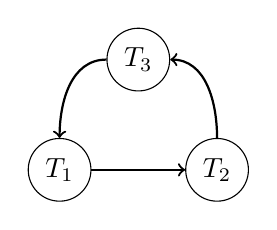
\begin{tikzpicture}
        [
            task/.style={circle, draw},
        ]
            \node[task] (T1) at (0.0, 0.0) {$T_1$};
            \node[task] (T2) at (2.0, 0.0) {$T_2$};
            \node[task] (T3) at (1.0, 1.4) {$T_3$};
            
            \draw[->, thick, draw] (T1.east) to [out=0,in=180] (T2.west);
            \draw[->, thick, draw] (T2.north) to [out=90,in=0] (T3.east);
            \draw[->, thick, draw] (T3.west) to [out=180,in=90] (T1.north);
        \end{tikzpicture}
        \caption{Precedence graph for schedule 1}
        \label{fig:trans-schedule-1}
    \end{figure}
    Since the graph forms a cycle, schedule 1 is not conflict serializable.

    \colbreak

    ...
    \begin{figure}[H]
        \centering
        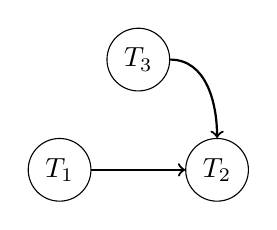
\begin{tikzpicture}
        [
            task/.style={circle, draw},
        ]
            \node[task] (T1) at (0.0, 0.0) {$T_1$};
            \node[task] (T2) at (2.0, 0.0) {$T_2$};
            \node[task] (T3) at (1.0, 1.4) {$T_3$};
            
            \draw[->, thick, draw] (T1.east) to [out=0,in=180] (T2.west);
            \draw[->, thick, draw] (T3.east) to [out=0,in=90] (T2.north);
        \end{tikzpicture}
        \caption{Precedence graph for schedule 2}
        \label{fig:trans-schedule-2}
    \end{figure}

\end{multicols}

%==============================================================================%
% OPTIMISTIC CONCURRENCY CONTROL                                               %
%==============================================================================%

\section{Optimistic Concurrency Control}
...

%==============================================================================%
% PROGRAMMING TASKS                                                            %
%==============================================================================%

\newpage
\section{Programming Tasks}

\setlength\columnsep{30pt}
\begin{multicols}{2}
    In order to implement the functionality, we added the message tags for the
    desired functions to {\tt BookStoreMessageTags} --- namely
    {\tt GETBOOKSINDEMAND}, {\tt RATEBOOKS} and {\tt GETTOPRATEDBOOKS}, as
    shown in excerpt \ref{code:utils/BookStoreMessageTag.java}.
    
    \colbreak
    
    \codeexcerpt{utils/BookStoreMessageTag.java}{12}{14}
\end{multicols}
\setlength\columnsep{10pt}

\subsection{\tt rateBooks}
The implementation of {\tt rateBooks} is rather straight forward. First we check
that the argument isn't null. Then, for each of the ratings passed to us, we
validate that the ISBN is valid and contained within the book map, and lastly
that the rating is actually valid. If any of these fails, we throw an exception.
If not, we proceed to perform the rating.
\codeexcerpt{business/CertainBookStore.java}{333}{370}

Now that the functionality is implemented, we can add the message handling code.

Firstly, we parse the serialized XML from the received POST request. Then we
attempt to perform the rating using the set of book ratings. If this fails we
catch the generated exception. And lastly, if all went well, we respond
accordingly.
\codeexcerpt{server/BookStoreHTTPMessageHandler.java}{251}{266}

Now the server is able to process book ratings, so all we have to do is to
expose the client-side to this API. To do so, we simply serialize the book
ratings and send the POST request with it and wait for a response from the
server.
\codeexcerpt{client/BookStoreHTTPProxy.java}{132}{144}

\subsection{\tt getTopRatedBooks}
To implement this, we first check that we are being asked for a valid number of
books to retrieve. If not, we produce an exception. Then we make a
{\tt Collection} containing the values of the book map, such that we can sort
the values based on the output of a {\tt Comparator} that compares the {\tt
getAverageRating} method. Once sorted, we merely need to cut the upper entries
of the resultant list to get the requested number of toprated books. We then
make a set of the ISBN numbers and use the {\tt getBooks} functionality to
produce and return the books.
\codeexcerpt{business/CertainBookStore.java}{280}{311}

The server now needs to recognize and handle the message. We do so by
extracting and decoding the {\tt BOOK\_NUM\_PARAM} parameter and pass it to the
book store object, which performs the retrieveal, and then we serialize the
returned object into XML and then write it to the response object.
\codeexcerpt{server/BookStoreHTTPMessageHandler.java}{268}{285}

To finish things up, we implement the client-side, which initiates the action.
In this, we encode the number of toprated books to be fetched and use it to
produce the URL parameter {\tt BOOK\_NUM\_PARAM}, and then sending the request
and wait for a response.
\codeexcerpt{client/BookStoreHTTPProxy.java}{148}{166}

\subsection{\tt getTopRatedBooks}
TODO: explain
\codeexcerpt{business/CertainBookStore.java}{313}{330}

%==============================================================================%
% DISCUSSION                                                                   %
%==============================================================================%

\section{Discussion on the Performance Measurements}
...

\subsection{Setup}
\dots

\subsection{Plots}
\dots

\subsection{Reliability}
\dots


\end{document}
